\documentclass[12pt,a4paper]{article}

\usepackage[utf8]{inputenc}
\usepackage[T2A]{fontenc}
\usepackage[russian]{babel}
\usepackage{amsmath,amssymb}
\usepackage{graphicx}
\usepackage{booktabs}
\usepackage{geometry}
\usepackage{float}
\usepackage{indentfirst}
\usepackage{siunitx}
\usepackage{pgfplots}
\pgfplotsset{compat=1.18}
\geometry{top=2cm,bottom=2cm,left=2.5cm,right=1.5cm}
\sisetup{output-decimal-marker={,}}

\title{\textbf{Лабораторная работа 1.2.5}\\
Исследование вынужденной регулярной прецессии гироскопа}
\author{
Студент: \underline{Шеховцов Василий Максимович}\\
Группа: \underline{Б03-601}\\
Преподаватель: \underline{Ивлев Д.А.}
}
\date{Московский Физико-технический институт\\
(национальный исследовательский университет)\\
21 октября 2026 г.}

\begin{document}
\maketitle

\section*{Цель работы}
Исследовать вынужденную регулярную прецессию гироскопа и проверить зависимость угловой скорости прецессии от момента внешних сил.

\section*{Оборудование}
Гироскоп с ротором, крутильный подвес, калибровочный цилиндр, набор грузов, секундомер, генератор сигнала и осциллограф.

\section*{Теоретическая часть}

При вращении гироскопа с угловой скоростью $\omega_0$ его момент импульса при вращении вокруг оси ротора равен
\[
L=I_0\omega_0,
\]
где $I_0$ --- момент инерции ротора относительно оси вращения.

Под действием момента внешних сил $\mathbf M$ направление вектора момента импульса изменяется. При регулярной прецессии модуль угловой скорости прецессии равен
\begin{equation}
\Omega=\frac{M}{I_0\omega_0}.
\label{eq:precession}
\end{equation}
Для подвешенного груза момент силы при перпендикулярном плече $l$:
\begin{equation}
M=mgl.
\label{eq:moment}
\end{equation}
Экспериментальную угловую скорость прецессии определяем по времени одного полного оборота:
\begin{equation}
\Omega_{\text{эксп}}=\frac{2\pi}{T}.
\label{eq:omegaexp}
\end{equation}

Момент инерции ротора определяем методом крутильных колебаний. Для ротора и калибровочного цилиндра, измеренных на одной установке,
\begin{equation}
I_0=I_{\text{ц}}\left(\frac{T_0}{T_{\text{ц}}}\right)^2,
\label{eq:inertia}
\end{equation}
где $T_0$ и $T_{\text{ц}}$ --- периоды крутильных колебаний ротора и калибровочного цилиндра. Для однородного сплошного цилиндра
\[
I_{\text{ц}}=\frac{m_{\text{ц}}R_{\text{ц}}^2}{2}.
\]
Угловая скорость ротора связана с частотой вращения соотношением
\begin{equation}
\omega_0=2\pi \nu.
\label{eq:spin}
\end{equation}

\section{Определение момента инерции ротора}

Масса калибровочного цилиндра $m_{\text{ц}}=1{,}6158$ кг, диаметр $d_{\text{ц}}=7{,}94$ см, поэтому $R_{\text{ц}}=0{,}0397$ м. Измерено время 15 крутильных колебаний: $60{,}30$, $59{,}91$ и $60{,}26$ с.

Момент инерции калибровочного цилиндра:
\[
I_{\text{ц}}=\frac{1}{2}\cdot1{,}6158\cdot(0{,}0397)^2
=1{,}2733\cdot10^{-3}\ \text{кг}\cdot\text{м}^2.
\]
Среднее время 15 колебаний равно
\[
\overline t_{\text{ц}}=\frac{60{,}30+59{,}91+60{,}26}{3}
=60{,}1567\ \text{с},
\]
откуда
\[
T_{\text{ц}}=\frac{60{,}1567}{15}=4{,}0104\ \text{с}.
\]

Для ротора получены измерения: 18 колебаний за $60{,}62$ с, 19 за $60{,}73$ с и 19 за $60{,}49$ с. По суммарному числу колебаний:
\[
T_0=\frac{60{,}62+60{,}73+60{,}49}{18+19+19}
=3{,}2471\ \text{с}.
\]
Тогда
\[
I_0=1{,}2733\cdot10^{-3}
\left(\frac{3{,}2471}{4{,}0104}\right)^2
=8{,}3475\cdot10^{-4}\ \text{кг}\cdot\text{м}^2.
\]

\subsection*{Проверка ротора с помощью формулы}
Масса ротора $m_0=1{,}0828$ кг, внешний диаметр $d_{\text{нар}}=6{,}86$ см, внутренний диаметр $d_{\text{вн}}=3{,}49$ см. Приближая ротор однородным полым цилиндром, получаем
\[
I=\frac{m_0}{2}
\left(R_{\text{нар}}^2+R_{\text{вн}}^2\right),
\]
где $R_{\text{нар}}=0{,}0343$ м и $R_{\text{вн}}=0{,}01745$ м. Следовательно,
\[
I\approx8{,}018\cdot10^{-4}\ \text{кг}\cdot\text{м}^2.
\]
Это примерно на $4{,}1\%$ меньше значения, найденного методом крутильных колебаний. Геометрическая оценка является приближённой, поэтому далее используем экспериментальное значение $I_0$.

\section{Частота вращения ротора}

По фигуре Лиссажу получено значение частоты около $390{,}6$ Гц, а частота генератора установлена равной $400$ Гц. Поэтому принимаем интервал
\[
390{,}6\leq \nu\leq400\ \text{Гц}.
\]
Соответствующая угловая скорость ротора находится в диапазоне
\[
\omega_0=2\pi \nu,\qquad
2454{,}4\leq\omega_0\leq2513{,}3\ \text{рад/с}.
\]
Для центральной оценки $\nu=395{,}3$ Гц получаем $\omega_0\approx2483{,}2$ рад/с.

\section{Измерение скорости прецессии}

Длина плеча $l=120$ мм $=0{,}120$ м. Каждое приведённое время соответствует одному полному обороту.
\begin{table}[H]
\centering
\caption{Исходные времена одного оборота}
\small
\begin{tabular}{c c c c c c c c}
\toprule
№ & $\varphi$, град & $m$, г & \multicolumn{5}{c}{Время оборота $T_i$, с}\\
\cmidrule(lr){4-8}
 & & & 1 & 2 & 3 & 4 & 5\\
\midrule
1 & 17 & 56,1 & 177,04 & 175,54 & 176,25 & 175,58 & ---\\
2 & 15 & 91,6 & 107,43 & 106,95 & 107,77 & 110,82 & 107,96\\
3 & 13 & 141,7 & 69,24 & 70,95 & 69,39 & 69,69 & 68,39\\
4 & 9 & 218,8 & 44,73 & 44,38 & 46,20 & 45,11 & 45,15\\
5 & 7 & 340,4 & 28,70 & 29,04 & 29,30 & 28,88 & 27,47\\
\bottomrule
\end{tabular}
\end{table}

Для каждого опыта вычисляем среднее время оборота $\overline T$, момент силы $M=mgl$ и экспериментальную скорость $\Omega_{\text{эксп}}=2\pi/\overline T$. Теоретическое значение рассчитываем по формуле (\ref{eq:precession}) для двух границ частоты:
\[
\Omega_{\text{теор}}(\nu)=\frac{mgl}{I_0\,2\pi \nu}.
\]

\begin{table}[H]
\centering
\caption{Сравнение экспериментальной и теоретической скорости прецессии}
\small
\begin{tabular}{c c c c c c}
\toprule
№ & $\overline T$, с & $M$, Н$\cdot$м & $\Omega_{\text{эксп}}$, рад/с &
$\Omega_{\text{теор}}(400)$ & $\Omega_{\text{теор}}(390{,}6)$\\
\midrule
1 & 176,103 & 0,06604 & 0,03568 & 0,03148 & 0,03224\\
2 & 108,186 & 0,10783 & 0,05808 & 0,05140 & 0,05264\\
3 & 69,532 & 0,16681 & 0,09036 & 0,07951 & 0,08142\\
4 & 45,114 & 0,25757 & 0,13927 & 0,12277 & 0,12573\\
5 & 28,678 & 0,40072 & 0,21909 & 0,19100 & 0,19560\\
\bottomrule
\end{tabular}
\end{table}

Относительное расхождение определяем по формуле
\[
\varepsilon=\frac{\Omega_{\text{эксп}}-\Omega_{\text{теор}}}
{\Omega_{\text{теор}}}\cdot100\%.
\]

\begin{figure}[H]
    \centering
    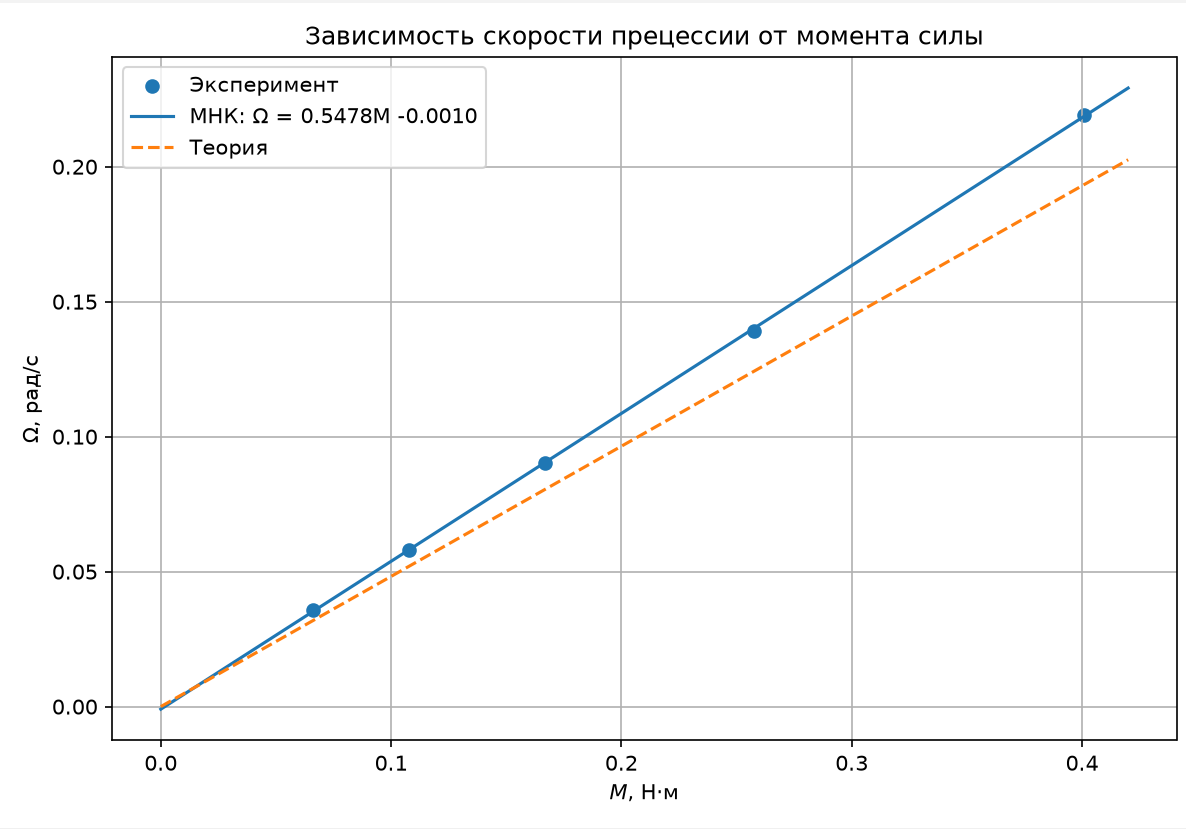
\includegraphics[width=0.85\textwidth]{graph.png}
    \caption{Зависимость угловой скорости прецессии от момента внешней силы}
    \label{fig:precession}
\end{figure}

жн
\section*{Вывод}

В работе экспериментально исследована вынужденная регулярная прецессия гироскопа. Момент инерции ротора, найденный по периоду крутильных колебаний, равен
\[
I_0\approx8{,}35\cdot10^{-4}\ \text{кг}\cdot\text{м}^2.
\]
При увеличении момента внешней силы от $0{,}0660$ до $0{,}4007$ Н$\cdot$м угловая скорость прецессии увеличилась от $0{,}0357$ до $0{,}2191$ рад/с, что согласуется с линейной зависимостью, следующей из теории. Экспериментальные значения превышают теоретические на $10$--$15\%$. 

\end{document}